\documentclass[11pt,a4paper]{article}
\usepackage[margin=25mm]{geometry}
\usepackage[T1]{fontenc}
\usepackage[utf8]{inputenc}
\usepackage{lmodern,microtype,amsmath,amssymb,bm,graphicx,booktabs,tabularx,array}
\usepackage{float}
\newfloat{algorithm}{htbp}{loa}
\floatname{algorithm}{Algorithm}
\usepackage[numbers,sort&compress]{natbib}
\usepackage{caption,subcaption,placeins,xcolor,etoolbox}
\usepackage[colorlinks=true,allcolors=blue!45!black]{hyperref}
\graphicspath{{figures/}}
 
\setlength{\emergencystretch}{2em}
\setlength{\parskip}{3pt}
\renewcommand{\topfraction}{0.95}
\renewcommand{\bottomfraction}{0.95}
\renewcommand{\textfraction}{0.05}
\renewcommand{\floatpagefraction}{0.75}
\captionsetup{font=small,labelfont=bf}
\newcommand{\RepositoryURL}{https://github.com/pv-emulation-lab/pv-bounded-residual-boosting}
\newcommand{\FundingStatement}{This research received no external funding.}
\newcommand{\ConflictStatement}{The authors declare no competing interests.}
\newcommand{\ContributionStatement}{A.L. and K.C. contributed equally to this work. A.L. and K.C. jointly conceptualized the study, designed the methodology, developed the software, performed the simulations and analysis, curated the data, prepared the figures, and wrote the original draft. A.Y. supervised the research, provided guidance on the methodology, reviewed and edited the manuscript, and administered the project. All authors read and approved the final manuscript.}
\newcommand{\unit}{\ensuremath{\mathrm{kWh\,day^{-1}\,kWp^{-1}}}}
\title{Bounded Residual Boosting for Daily Photovoltaic Energy Emulation Using Local NASA POWER Data: A Case Study of Cagayan de Oro City, Philippines}
\author{Ar-gie Longganay\textsuperscript{1}, Kaiser Cultura\textsuperscript{1}, and Abid Yahya\textsuperscript{2,*}}
\date{}
\begin{document}
\maketitle
\vspace{-1.3em}
\begin{center}\small
\textsuperscript{1}Department of Electrical Engineering, University of Science and Technology of Southern Philippines, Cagayan de Oro City 9000, Philippines\\
\textsuperscript{2}Department of Electrical Engineering, Botswana International University of Science and Technology, Palapye, Botswana\\
\textsuperscript{*}Correspondence: Abid Yahya, \href{mailto:yahyabid@gmail.com}{yahyabid@gmail.com}
\end{center}
\begin{abstract}
Daily photovoltaic emulators can appear limited by the learning algorithm when their inputs omit irradiance information used to generate the reference output. This study examines that distinction using 43,824 hourly NASA POWER records for Cagayan de Oro, Philippines, and a reproducible pvlib simulation of a generic 1-kWp array. A bounded residual-boosting model combines a calibrated plane-of-array energy anchor with daily irradiation, temperature and wind moments. The formulation is evaluated against daily-weather regressors, direct boosting with matched inputs, and a plane-of-array ratio estimator. Hyperparameters are selected on 2024 after fitting on 2021--2023; final models use 2021--2024 and are evaluated on 365 days in 2025. The moment-based residual model attains a mean absolute error of 0.01049~\unit{} and $R^2=0.99968$, compared with 0.26115 for daily-weather XGBoost, 0.05300 for the physical ratio estimator, and 0.01961 for direct boosting with the same moment inputs. Paired month-block resampling supports the reduction relative to these comparators. Adding irradiance-closure discrepancies does not improve the moment-based residual model. Recomputing direct normal irradiance changes both the reference energy and its emulation difficulty, so that intervention cannot establish which irradiance product is more accurate. The results identify the value of preserving subdaily irradiance structure when emulating a deterministic photovoltaic model. They are retrospective simulator experiments, without measured-production validation or a demonstrated computational advantage over pvlib.
\end{abstract}
\noindent\textbf{Keywords:} photovoltaic emulation; residual boosting; irradiance aggregation; physical moments; chronological evaluation; NASA POWER.

\section{Introduction}
Photovoltaic energy estimation depends on two distinct mappings: the atmospheric conditions that determine irradiance, and the optical, thermal and electrical processes that convert irradiance into production. Forecasting studies must additionally specify when their input information becomes available. Reviews distinguish direct statistical forecasts from indirect approaches that first estimate irradiance and then apply a photovoltaic conversion model \cite{antonanzas2016}. That distinction is essential when interpreting models trained on simulated energy.

A simulator-generated target permits reproducible experiments under controlled assumptions, but it also creates an information problem. A photovoltaic simulator may use hourly global horizontal irradiance (GHI), direct normal irradiance (DNI), diffuse horizontal irradiance (DHI), solar geometry, temperature and wind. An emulator given only daily GHI and mean weather cannot generally reconstruct that hourly input state. Poor agreement may therefore reflect aggregation and omitted information rather than an unsuitable regression algorithm.

The initial benchmark for Cagayan de Oro exhibits precisely this pattern. Daily-weather XGBoost approximates the reference reasonably well, yet a one-coefficient estimator using plane-of-array (POA) irradiation is substantially more accurate. The useful research question is consequently whether a compact physical representation can retain the information needed for accurate daily emulation, and whether residual learning adds value once the input representation is controlled.

Hybrid photovoltaic methods already combine physical models and statistical learning \cite{santos2024}. More recently, Ou Yang et al.\ use a physical baseline and an attention-based sequence model for four-hour-ahead forecasting \cite{ouyang2026}. Residual correction is therefore an established construction. The present contribution is its explicit use within an information-controlled daily emulation audit: a POA anchor, physically motivated subdaily moments, matched-input direct and residual regressors, bounded reconstruction, and a separate irradiance-intervention experiment. The proposed combination is evaluated on the supplied archive; no claim is made that residual learning, boosting, or physical constraints are individually new.

The study has three objectives. First, it measures how much error is associated with a daily-weather representation relative to a component-aware representation. Second, it tests whether learning deviations from a physical energy anchor improves on learning total energy with identical predictors. Third, it distinguishes diagnostic closure discrepancies from evidence about the accuracy of gridded irradiance. The site is the USTP Cagayan de Oro campus, but the weather represents a grid cell and the photovoltaic system is hypothetical. All outputs discussed below are simulated energy, rather than campus meter readings.

\section{Related work and study position}
Open photovoltaic modeling libraries make the conversion chain inspectable. The original pvlib-python publication \cite{holmgren2018} and its project update \cite{anderson2023} describe implementations of solar-position, irradiance, thermal and electrical models. PVWatts provides a documented simplified electrical formulation \cite{dobos2014}. These tools support reproducibility, while agreement with them measures emulation fidelity rather than field accuracy.

The review by Santos et al.\ distinguishes several ways to integrate physics and learning \cite{santos2024}. A physical variable can enter a statistical predictor, or a statistical model can correct a physical estimate. The present study explicitly implements both routes. Direct and residual boosting share the same input moments, which allows their difference to be assessed without confusing it with access to additional information. XGBoost supplies the regularized tree learner \cite{chen2016}; random forests supply a conventional daily-weather comparator \cite{breiman2001}.

Philippine photovoltaic forecasting has also been studied using SARIMAX, recurrent networks and XGBoost \cite{benitez2023}. Those results address future measured output and cannot be numerically ranked against contemporaneous simulator emulation. Here, the realized weather of the estimated day is available to every relevant model. No day-ahead forecasting claim follows from the reported errors.

NASA POWER documents the irradiance-component products and their corrections separately \cite{power,powercomponents}. This matters because a discrepancy between downloaded hourly components and a locally calculated instantaneous geometry is not, by itself, evidence of erroneous source observations. Time-series assessment also requires care: empirical work shows that temporal dependence and non-stationarity affect performance estimation \cite{cerqueira2020}. The protocol therefore keeps fitting and selection earlier than the evaluation year, and treats historical windows and test-year resampling as conditional diagnostics.

\section{Data and physical reference}
\subsection{Weather archive and time handling}
The supplied archive contains seven hourly variables from NASA POWER for 1 January 2021 through 31 December 2025 in UTC. The request uses community RE, latitude $8.486^{\circ}$ N, longitude $124.657^{\circ}$ E, and the hourly point endpoint. Archived response headers identify SYN1DEG, MERRA2 and POWER as sources and record a download date of 31 October 2026. Table~\ref{tab:data} summarizes the provenance and chronological partitions.
\begin{table}[htbp]\centering\small
\caption{Data provenance, time conventions and model partitions.}\label{tab:data}
\begin{tabularx}{\linewidth}{@{}lX@{}}\toprule
Item & Specification\\\midrule
Coordinates and elevation & $8.486^{\circ}$ N, $124.657^{\circ}$ E; grid elevation 113.37 m\\
Hourly archive & 43,824 records; seven variables; UTC; no missing hours or fill values\\
Irradiance variables & ALLSKY\_SFC\_SW\_DWN, ALLSKY\_SFC\_SW\_DNI, ALLSKY\_SFC\_SW\_DIFF\\
Meteorological variables & T2M, RH2M, WS10M, PRECTOTCORR\\
Daily aggregation & Philippine Standard Time, UTC+08:00; complete 24-hour days only\\
Retained daily records & 1,825 days: 2 January 2021--31 December 2025\\
Initial fitting & 2021--2023: 1,094 days\\
Hyperparameter selection & 2024: 366 days\\
Final fitting / evaluation & 2021--2024: 1,460 days / 2025: 365 days\\\bottomrule
\end{tabularx}\end{table}

The archive has no duplicated timestamps or $-999$ fill values; no imputation is used. Hourly irradiance entries are supplied in Wh/m$^2$ over one-hour intervals. Their numerical values therefore equal the corresponding interval-mean W/m$^2$ values used in the simulator. This equality depends on the one-hour duration and must not be carried over to other resolutions without conversion. Precipitation rates in mm/h are multiplied by the one-hour duration before summation. The first and last local days are incomplete after converting from UTC and are excluded.

Solar geometry is evaluated at the midpoint of each one-hour interval, while energy is grouped by the local date of its interval start. The two dates agree for every retained interval. The complete energy record and the monthly distribution of the POA-to-horizontal irradiation ratio are shown in Figure~\ref{fig:record}. The latter ratio illustrates a component of the optical geometry that a daily GHI total alone does not identify.
\begin{figure}[htbp]\centering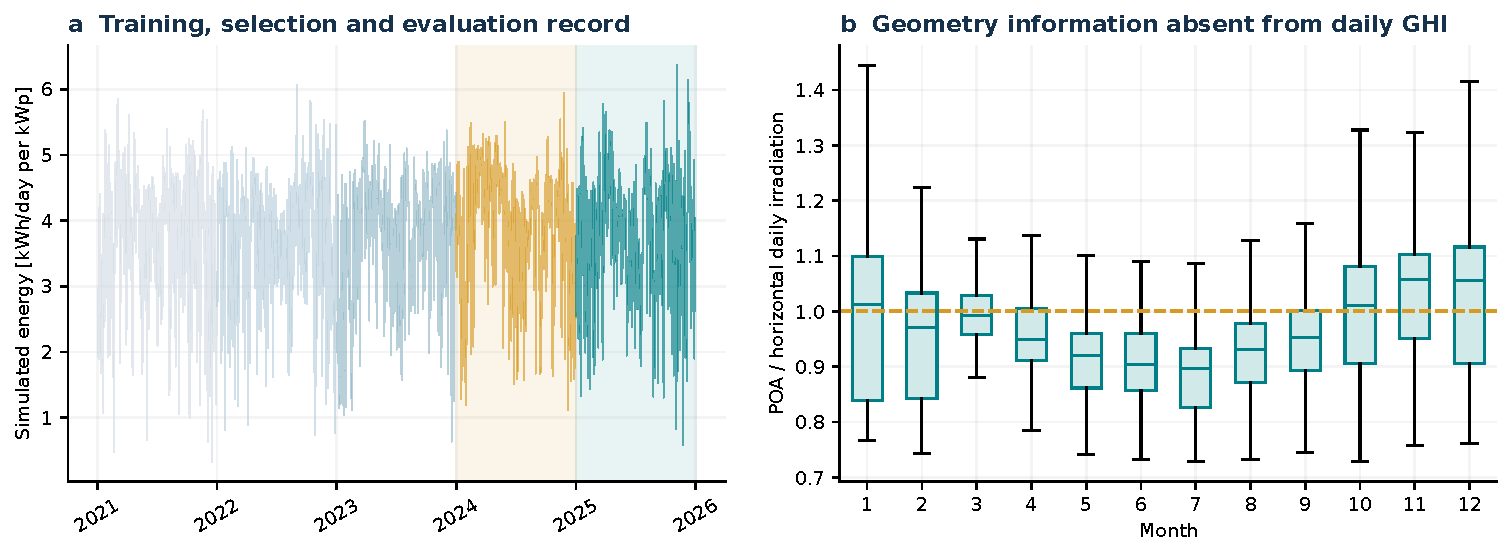
\includegraphics[width=\linewidth]{reference-record.pdf}
\caption{Simulated daily reference and irradiation geometry. (a) Energy record with 2024 selection and 2025 evaluation periods shaded. (b) Monthly distributions of POA-to-horizontal daily irradiation over the five-year record; boxes show quartiles, with conventional 1.5-interquartile-range whiskers and outliers suppressed.}\label{fig:record}\end{figure}

\subsection{Reference conversion chain}
The configuration in Table~\ref{tab:system} is implemented using pvlib 0.16.1. The simulated array has no site-specific shading, measured soiling trajectory, curtailment or degradation model. Default PVWatts losses are retained. Those defaults already include generic loss categories, including shading and availability, so the reference should not be described as excluding all such losses.
\begin{table}[htbp]\centering\small
\caption{Fixed generic photovoltaic reference configuration.}\label{tab:system}
\begin{tabularx}{\linewidth}{@{}lX@{}}\toprule
Component & Value or model\\\midrule
DC nameplate & $P_0=1$ kWp at standard test conditions\\
Array geometry & Fixed tilt $10^{\circ}$; azimuth $180^{\circ}$; albedo 0.2\\
Transposition & Perez, with pvlib ModelChain PVWatts configuration\\
Thermal model & SAPM, open-rack glass/polymer parameters\\
Optical / spectral treatment & Physical angle-of-incidence loss / no spectral correction\\
DC conversion & PVWatts; temperature coefficient $-0.0035$ K$^{-1}$\\
Inverter parameters & $p_{\mathrm{dc},0}=1000/1.1$ W; nominal efficiency 0.96\\
Actual AC ceiling & $0.96(1000/1.1)=872.727$ W\\
System losses & pvlib default PVWatts loss set, approximately 14.08\%\\\bottomrule
\end{tabularx}\end{table}

Let $\mathcal H_d$ denote the 24 hourly intervals belonging to local day $d$, and let $I_h$ be POA irradiance in kW/m$^2$. The daily target per unit DC capacity is
\begin{equation}
 E_d=\frac{1}{P_0}\sum_{h\in\mathcal H_d}\max(P_{\mathrm{ac},h},0)\Delta t,
 \qquad \Delta t=1\ \mathrm{h}.
 \label{eq:energy}
\end{equation}
Here $P_{\mathrm{ac},h}$ is expressed in kW and $P_0$ in kWp. The implementation clips negative nighttime inverter output to zero. Rerunning the supplied physical chain reproduces the archived daily reference with a maximum absolute difference of $8.9\times10^{-16}$~\unit{}.

The distinction between the inverter's DC input rating and its AC ceiling is consequential. The parameter $1000/1.1$ W is the PVWatts inverter DC reference, not its delivered AC limit. For this configuration the modeled maximum AC output is 872.727 W. A conservative daily upper bound is therefore
\begin{equation}
 U=24\,\frac{0.96}{1.1}=20.94545\ \unit{}.
 \label{eq:bound}
\end{equation}
This bound is deliberately loose because it allows full inverter output throughout all 24 hours; it is a feasibility guard rather than a tight solar-resource envelope.

\section{Bounded residual boosting}
\subsection{Daily inputs and physical moments}
The daily-weather feature vector is
\begin{equation}
 \bm x_d=(H_{\mathrm{GHI},d},\bar T_d,\overline{\mathrm{RH}}_d,\bar v_d,R_d,
 \sin(2\pi j_d/365.25),\cos(2\pi j_d/365.25)),
 \label{eq:daily}
\end{equation}
where $R_d$ is daily precipitation and $j_d$ is the day of year. It has seven predictors. The proposed representation adds four quantities computed from hourly weather and optical transposition:
\begin{align}
 H_d&=\sum_{h\in\mathcal H_d} I_h\Delta t, &
 M_{2,d}&=\sum_{h\in\mathcal H_d} I_h^2\Delta t,\nonumber\\
 M_{T,d}&=\sum_{h\in\mathcal H_d} I_h(T_{a,h}-25)\Delta t, &
 M_{v,d}&=\sum_{h\in\mathcal H_d} I_hv_h\Delta t.
 \label{eq:moments}
\end{align}
The resulting vector $\bm z_d=(\bm x_d,H_d,M_{2,d},M_{T,d},M_{v,d})$ has 11 predictors. Its inputs contain neither AC output nor cell temperature. The optical preprocessing uses pvlib's input-preparation routine; the electrical reference is used only to construct training responses and evaluate predictions.

These moments have a physical motivation. A simplified temperature-sensitive conversion can be written
\begin{equation}
 P_{\mathrm{dc},h}\ \propto\ I_h\{1+\gamma(T_{c,h}-25)\},\qquad
 T_{c,h}\approx T_{a,h}+aI_h-bv_h.
 \label{eq:approx}
\end{equation}
After summation, the leading terms depend on $H_d$, $M_{T,d}$, $M_{2,d}$ and $M_{v,d}$. Equation~\eqref{eq:approx} motivates the representation; it is not substituted for SAPM in the reference simulator, and $a$ and $b$ are not fitted physical parameters in the proposed method. The moment vector retains irradiance intensity and its coincidence with temperature and wind, which daily means discard. It does not reconstruct the full hourly sequence.

\subsection{Anchor, residual objective and projection}
For a fitting set $\mathcal T$, define the energy-conserving ratio anchor and its residual target as
\begin{equation}
 \widehat k_{\mathcal T}=\frac{\sum_{d\in\mathcal T}E_d}{\sum_{d\in\mathcal T}H_d},\qquad
 b_d=\widehat k_{\mathcal T}H_d,\qquad r_d=E_d-b_d.
 \label{eq:anchor}
\end{equation}
The coefficient is a ratio-of-sums calibration, rather than a least-squares slope. It ensures $\sum_{\mathcal T}r_d=0$. Calibration and residual construction are repeated within each fitting partition so that validation responses do not enter the anchor.

The correction is a regularized tree ensemble $g(\bm z)=\sum_{m=1}^{M}\eta f_m(\bm z)$ fitted to the residuals. Its squared-error objective follows the XGBoost construction \cite{chen2016}:
\begin{equation}
 \mathcal L(g)=\sum_{d\in\mathcal T}\tfrac12[r_d-g(\bm z_d)]^2+
 \sum_{m=1}^{M}\left(\alpha L_m+\tfrac{\lambda}{2}\|\bm w_m\|_2^2\right),
 \label{eq:objective}
\end{equation}
where $L_m$ is the number of leaves and $\bm w_m$ their scores. Here $\alpha=0$ and $\lambda=1$, consistent with the learner defaults; $\eta$ is selected from the stated grid. At each boosting step, the optimal unshrunk score for leaf $\ell$ is
\begin{equation}
 w_\ell^{*}=-\frac{G_\ell}{S_\ell+\lambda},\qquad
 G_\ell=\sum_{d\in\ell}(g_{\mathrm{old}}(\bm z_d)-r_d),\quad S_\ell=|\ell|.
 \label{eq:leaf}
\end{equation}
Subsampling uses 80\% of fitting rows per boosting iteration. The estimate is reconstructed by
\begin{equation}
 \widehat E_d=\Pi_{[0,U]}\{b_d+g(\bm z_d)\},\qquad
 \Pi_{[0,U]}(u)=\min(U,\max(0,u)).
 \label{eq:projection}
\end{equation}
For any valid reference $E_d\in[0,U]$, projection satisfies
\begin{equation}
 |\Pi_{[0,U]}(u)-E_d|\leq |u-E_d|.
 \label{eq:nonexpansive}
\end{equation}
This follows by considering $u<0$, $u\in[0,U]$ and $u>U$ separately. It guarantees feasibility and cannot increase pointwise absolute or squared error against a reference within the interval. It does not guarantee that residual learning improves on the physical anchor. Projection is inactive for the evaluated predictions, so the observed accuracy gain is not attributed to clipping.

Figure~\ref{fig:architecture} separates the predictor and target branches. Figure~\ref{fig:flow} and Algorithm~\ref{alg:training} specify the fitting and selection procedure.
\begin{figure}[htbp]\centering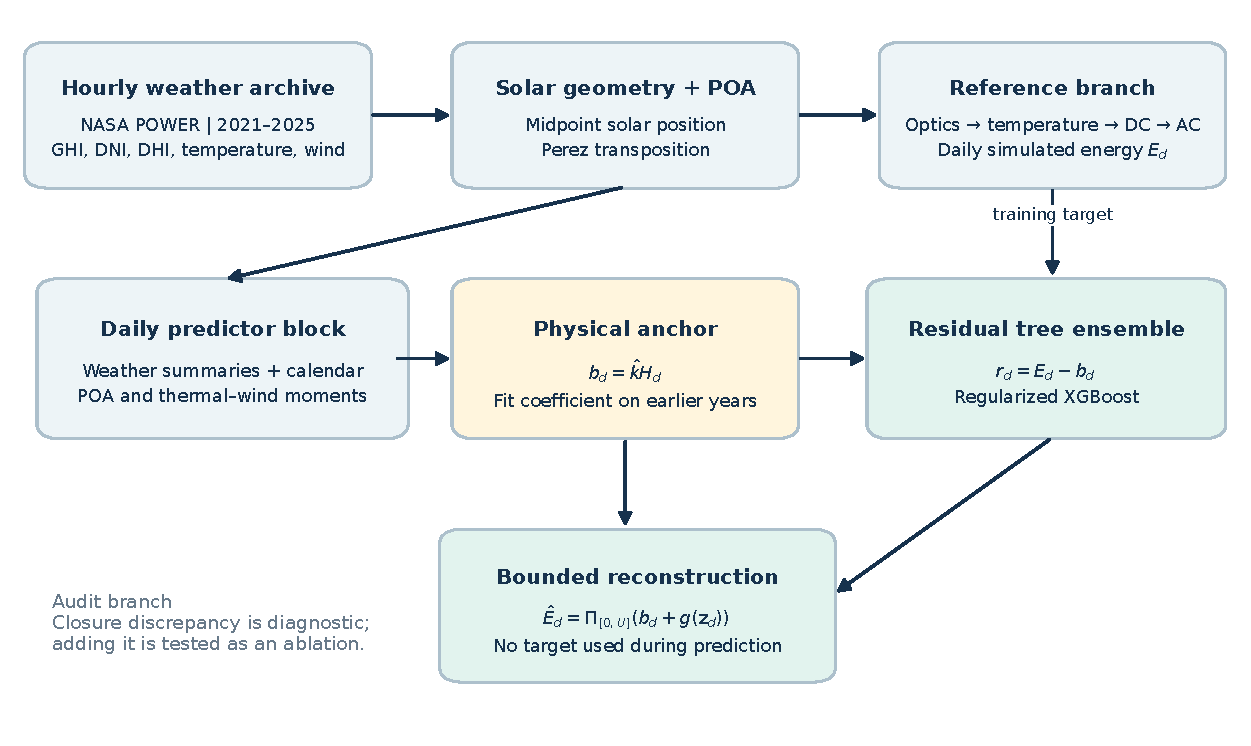
\includegraphics[width=\linewidth]{architecture.pdf}
\caption{Physical anchor and bounded residual architecture. Hourly optical preprocessing supplies POA irradiation and moments; the electrical simulation supplies training responses. The prediction branch does not use the response of the estimated day. Closure discrepancies are retained for diagnostics and a separate input ablation.}\label{fig:architecture}\end{figure}
\begin{figure}[htbp]\centering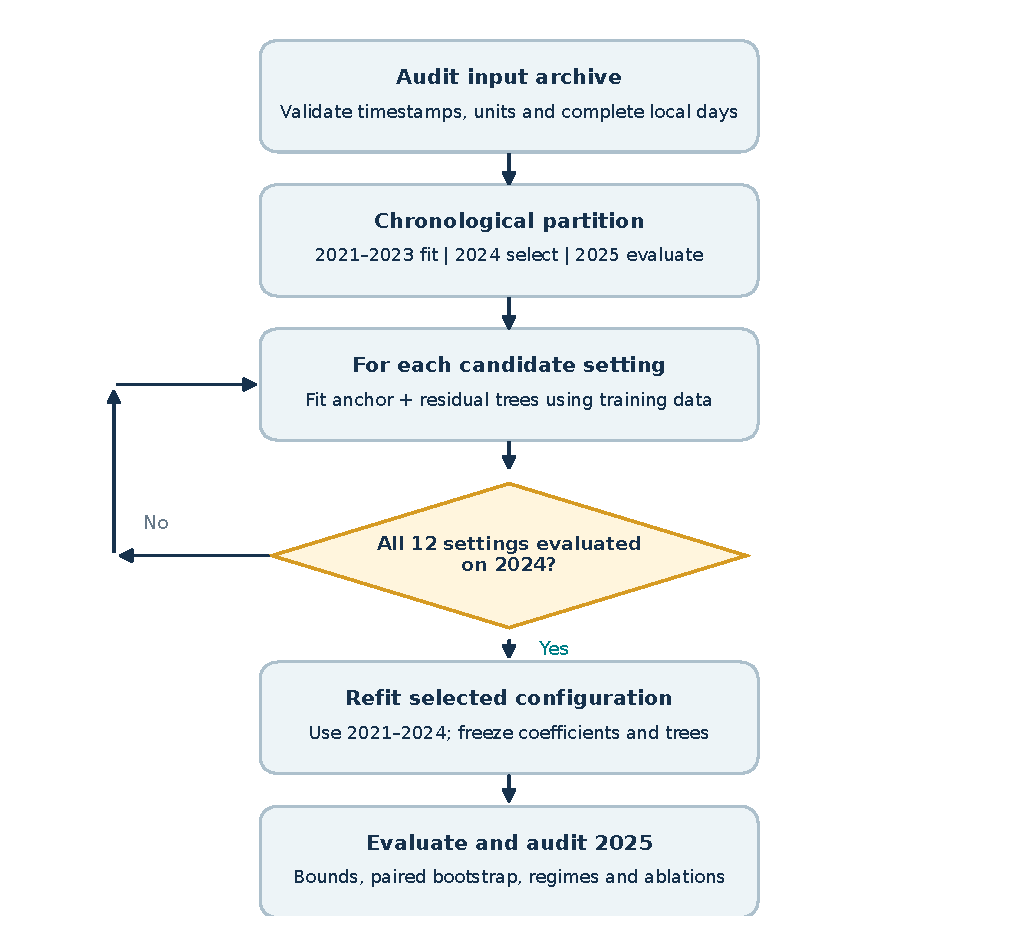
\includegraphics[width=.95\linewidth]{algorithm-flowchart.pdf}
\caption{Chronological fitting and selection flow. All candidate settings are evaluated on 2024 before the selected model is refitted on 2021--2024. The analysis is a retrospective extension of an existing benchmark, rather than a preregistered evaluation.}\label{fig:flow}\end{figure}
\begin{algorithm}[htbp]
\caption{Bounded residual boosting with moment inputs}\label{alg:training}
\small
\noindent\textbf{Input:} hourly weather, fixed PV configuration, candidate set $\mathcal Q$.
\begin{enumerate}\setlength{\itemsep}{2pt}
\item Audit timestamps, units and completeness; retain complete local days.
\item Compute responses $E_d$, POA irradiation $H_d$, and moment inputs $\bm z_d$.
\item Partition $\mathcal T=2021$--$2023$, $\mathcal V=2024$, $\mathcal S=2025$.
\item For each $q\in\mathcal Q$:
  \begin{enumerate}\setlength{\itemsep}{1pt}
  \item Fit $\widehat k_{\mathcal T}$ by Eq.~\eqref{eq:anchor}.
  \item Fit $g_q$ to $(\bm z_d,E_d-\widehat k_{\mathcal T}H_d)$ for $d\in\mathcal T$.
  \item Record RMSE of projected predictions on $\mathcal V$.
  \end{enumerate}
\item Select $q^*$ with minimum validation RMSE.
\item Refit the anchor and $g_{q^*}$ on $\mathcal T\cup\mathcal V$.
\item Freeze the fitted model; predict $\mathcal S$ using Eq.~\eqref{eq:projection}.
\item Evaluate errors, paired intervals, regimes and ablations.
\end{enumerate}

\end{algorithm}

\subsection{Closure discrepancy and intervention}
At an instant the horizontal component relationship involves $\mathrm{GHI}=\mathrm{DHI}+\mathrm{DNI}\cos\theta_z$. For the hourly archive define the numerical discrepancy
\begin{equation}
 q_h=\overline{\mathrm{GHI}}_h-\overline{\mathrm{DHI}}_h-
 \overline{\mathrm{DNI}}_h\max(\cos\theta_{z,h}^{\mathrm{mid}},0),\quad
 Q_d^{\pm}=10^{-3}\sum_h q_h\Delta t,\quad Q_d^{a}=10^{-3}\sum_h|q_h|\Delta t.
 \label{eq:closure}
\end{equation}
Hourly-mean products need not satisfy the instantaneous expression at a midpoint because $\overline{\mathrm{DNI}\cos\theta_z}$ generally differs from $\overline{\mathrm{DNI}}\cos\theta_z^{\mathrm{mid}}$. Component corrections documented by NASA POWER introduce a further product-processing consideration \cite{powercomponents}. Accordingly, $Q_d^{a}$ is an audit statistic and not a measured irradiance error.

A separate intervention replaces DNI by
\begin{equation}
 \mathrm{DNI}'_h=\begin{cases}
 \operatorname{clip}\!\left(\dfrac{\mathrm{GHI}_h-\mathrm{DHI}_h}{\cos\theta_{z,h}},0,1400\right),&\cos\theta_{z,h}>0.1,\\
 0,&\text{otherwise},
 \end{cases}\label{eq:intervention}
\end{equation}
with irradiance in W/m$^2$. The simulator and input features are recomputed, and models are refitted using their previously selected settings. Thresholding and clipping mean that even this intervention does not impose exact closure at every hour. It changes the simulated response as well as its input structure and is not a correction validated against ground observations.

\section{Experimental protocol}
\subsection{Comparators, ablations and selection}
All response-dependent transformations use only the corresponding fitting partition. Calendar means, GHI and POA ratio coefficients, and the regression models are refitted on 2021--2024 for final evaluation. Table~\ref{tab:models} defines the input and learning ablations; their purpose is to avoid presenting richer physical inputs as a pure algorithm improvement.
\begin{table}[htbp]\centering\small
\caption{Comparator and ablation definitions. ``Closure'' adds $Q_d^{\pm}$ and $Q_d^{a}$ from Eq.~\eqref{eq:closure}.}\label{tab:models}
\begin{tabularx}{\linewidth}{@{}lXl@{}}\toprule
Model & Input representation & Learned response\\\midrule
Calendar & Month index & Monthly mean energy\\
GHI ratio & Daily horizontal irradiation & One ratio coefficient\\
Daily linear / RF / XGBoost & Seven daily-weather/calendar features & Total energy\\
POA ratio & $H_d$ & One ratio coefficient\\
Direct / moments & $\bm z_d$, 11 features & Total energy\\
Direct / moments + closure & $\bm z_d$, closure; 13 features & Total energy\\
Residual / POA & $\bm x_d$, $H_d$; 8 features & Anchor residual\\
Residual / moments (proposed) & $\bm z_d$, 11 features & Anchor residual\\
Residual / moments + closure & $\bm z_d$, closure; 13 features & Anchor residual\\\bottomrule
\end{tabularx}\end{table}

Each boosted model is selected independently using the same 12-setting grid: $M\in\{200,500\}$ trees, depth in $\{3,5,7\}$ and learning rate in $\{0.03,0.1\}$. Row subsampling is 0.8, column subsampling is 1, minimum child weight is 1, $L_2$ regularization is 1, and the random seed is 42. Selection minimizes 2024 RMSE after fitting on 2021--2023. Linear regression uses an intercept. The random-forest comparator uses 500 trees, unrestricted depth and a minimum leaf size of three; it is a fixed conventional comparator, rather than the focus of a new tuning claim. Selected boosted settings are reported in Table~\ref{tab:tuning}.

The moment-based residual architecture has lower validation RMSE than its closure-augmented counterpart and is the primary configuration. The archive already contained 2025 benchmark results before this extension was designed. Thus, although this implementation selects its hyperparameters without fitting to 2025 responses, the overall study is retrospective. The 2025 evaluation is not presented as a previously unseen, confirmatory test of an independently preregistered method.

\subsection{Metrics and paired uncertainty}
For $n$ evaluation days and $e_d=\widehat E_d-E_d$, the reported statistics are
\begin{align}
 \mathrm{MAE}&=n^{-1}\sum_d|e_d|,&
 \mathrm{RMSE}&=\sqrt{n^{-1}\sum_de_d^2},\nonumber\\
 \mathrm{ME}&=n^{-1}\sum_de_d,&
 R^2&=1-\frac{\sum_de_d^2}{\sum_d(E_d-\bar E)^2}.
 \label{eq:metrics}
\end{align}
Mean error (ME) is positive for overestimation. MAE, RMSE and ME use \unit{}. Relative MAE reductions are computed as $1-\mathrm{MAE}_{\mathrm{proposed}}/\mathrm{MAE}_{\mathrm{comparator}}$.

Month-block resampling draws 12 months with replacement from the 12 observed months in 2025, retaining each selected month's complete daily sequence. There are 2,000 resamples with seed 42. Resampled day counts can vary because months have unequal lengths. Percentile intervals use the 2.5th and 97.5th percentiles. For model pairs, both errors are evaluated on exactly the same resampled days. These are conditional uncertainty summaries for this test-year record: they do not include parameter-selection uncertainty, preserve only within-month dependence, and have only 12 distinct blocks.

\subsection{Regimes and retrospective windows}
The absolute closure discrepancy $Q_d^a$ is divided into low, middle and high groups using the 2021--2024 tertiles, 0.4153 and 0.6759 kWh/m$^2$/day. Rainy days have at least 10 mm precipitation; hot days exceed the training-period 90th temperature percentile. Groups overlap, and no formal causal interpretation or independent significance claim is assigned to their differences.

An expanding-window diagnostic fits each model to earlier years and evaluates the next year from 2022 to 2025. Hyperparameters remain those selected using 2024. Consequently, the 2022--2024 windows are retrospective stability diagnostics, not nested prospective validation. A future multi-site study should nest hyperparameter selection inside every historical training window.

\section{Results}
\subsection{Selected settings and overall approximation}
\begin{table}[htbp]\centering\small
\caption{Selected boosted-model settings and validation RMSE. Fitting uses 2021--2023; selection uses 2024.}\label{tab:tuning}
\begin{tabular}{@{}lrrrr@{}}\toprule
Model & Trees & Depth & Learning rate & Validation RMSE\\\midrule
Daily XGBoost & 200 & 3 & 0.03 & 0.30436 \\
Direct / moments & 200 & 7 & 0.10 & 0.02707 \\
Direct / moments + closure & 500 & 3 & 0.03 & 0.02735 \\
Residual / POA & 200 & 5 & 0.03 & 0.02790 \\
Residual / moments & 500 & 3 & 0.03 & 0.02004 \\
Residual / moments + closure & 500 & 3 & 0.03 & 0.02131 \\
\bottomrule\end{tabular}\end{table}

Table~\ref{tab:performance} reports the 2025 results, with interval and error-distribution views in Figure~\ref{fig:performance}. The proposed moment-based residual model has MAE 0.01049, RMSE 0.01803 and $R^2=0.99968$. Its MAE interval is [0.00957, 0.01146]. Relative to daily-weather XGBoost, its MAE is 96.0\% lower. This comparison combines a richer input representation with a different response parameterization; it is not an estimate of the isolated value of residual learning.

\begin{table}[htbp]\centering\small
\caption{Chronological 2025 evaluation against simulated energy. Error statistics are in \unit{}. Brackets show 95\% month-block MAE intervals.}\label{tab:performance}
\begin{tabular}{@{}lrrrrl@{}}\toprule
Model & MAE & RMSE & ME & $R^2$ & MAE interval\\\midrule
Calendar & 0.80047 & 0.99379 & -0.01380 & 0.02755 & [0.71420, 0.88851] \\
GHI ratio & 0.37487 & 0.49141 & -0.03616 & 0.76222 & [0.32798, 0.42443] \\
Daily linear & 0.28993 & 0.39362 & -0.03160 & 0.84744 & [0.25657, 0.31904] \\
Daily RF & 0.26741 & 0.37237 & -0.02712 & 0.86347 & [0.24537, 0.28661] \\
Daily XGBoost & 0.26115 & 0.36490 & -0.03396 & 0.86889 & [0.23798, 0.28118] \\
POA ratio & 0.05300 & 0.07571 & +0.00603 & 0.99436 & [0.04837, 0.05748] \\
Direct / moments & 0.01961 & 0.04516 & -0.00572 & 0.99799 & [0.01623, 0.02314] \\
Direct / moments + closure & 0.01869 & 0.04015 & -0.00399 & 0.99841 & [0.01538, 0.02218] \\
Residual / POA & 0.01613 & 0.03094 & +0.00149 & 0.99906 & [0.01336, 0.01878] \\
Residual / moments & 0.01049 & 0.01803 & +0.00022 & 0.99968 & [0.00957, 0.01146] \\
Residual / moments + closure & 0.01090 & 0.01840 & -0.00042 & 0.99967 & [0.00962, 0.01211] \\
\bottomrule\end{tabular}\end{table}

The POA ratio anchor alone has MAE 0.05300. Adding the proposed residual correction reduces that value by 80.2\%. A stricter comparison uses direct boosting with the identical 11 moment inputs: its MAE is 0.01961, compared with 0.01049 for residual boosting, a 46.5\% reduction. That comparison supports an incremental benefit from the anchor-plus-residual formulation for this dataset, beyond access to hourly physical information.

\begin{figure}[htbp]\centering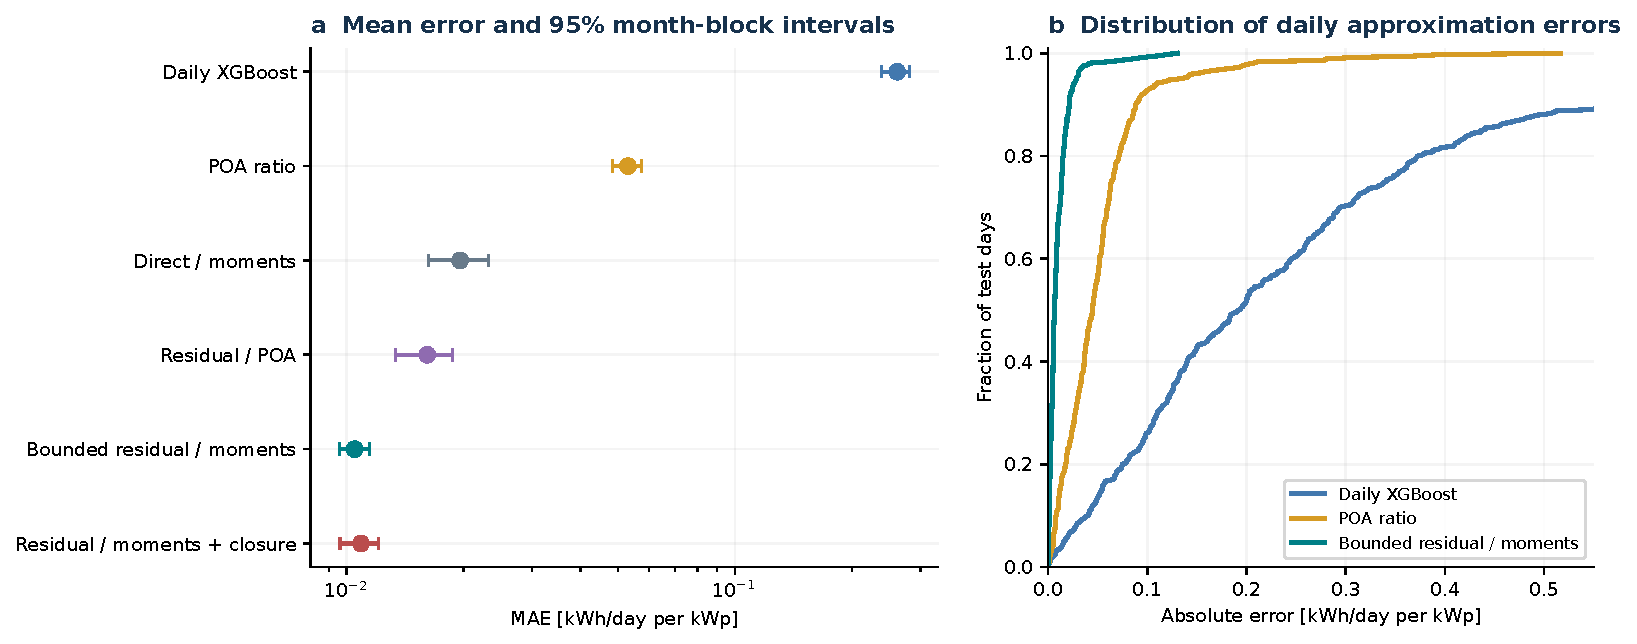
\includegraphics[width=\linewidth]{performance.pdf}
\caption{Evaluation against the simulated 2025 reference. (a) MAE and month-block intervals on a logarithmic error axis. (b) Empirical cumulative distribution of absolute daily errors; curves further left indicate smaller errors. The plotted cumulative distribution is restricted horizontally for readability.}\label{fig:performance}\end{figure}

Table~\ref{tab:paired} reports paired MAE differences. The intervals exclude zero for the comparisons with daily-weather XGBoost, the POA ratio, matched-input direct boosting and the reduced residual/POA model. These results summarize conditional differences within one evaluation year and do not establish a population-wide ranking.

\begin{table}[htbp]\centering\small
\caption{Paired MAE difference: proposed moment-based residual model minus comparator. Negative values favor the proposed model; all entries are in \unit{}.}\label{tab:paired}
\begin{tabular}{@{}lrrr@{}}\toprule
Comparator & Difference & Lower 95\% & Upper 95\%\\\midrule
Daily XGBoost & -0.25066 & -0.27036 & -0.22771 \\
POA ratio & -0.04251 & -0.04633 & -0.03862 \\
Direct / moments + closure & -0.00820 & -0.01141 & -0.00538 \\
Direct / moments & -0.00911 & -0.01241 & -0.00626 \\
Residual / POA & -0.00564 & -0.00790 & -0.00345 \\
\bottomrule\end{tabular}\end{table}

\subsection{Error structure and representation ablations}
The error atlas in Figure~\ref{fig:atlas} shows that daily-weather XGBoost errors are not distributed uniformly. Large signed errors occur on a subset of high-energy days and increase with the audit discrepancy. The moment-based residual model substantially compresses that pattern on the same color scale. Residual scatter is still present, especially for unusual high-energy conditions; low overall error should not be read as exact reproduction of every simulated day.
\begin{figure}[htbp]\centering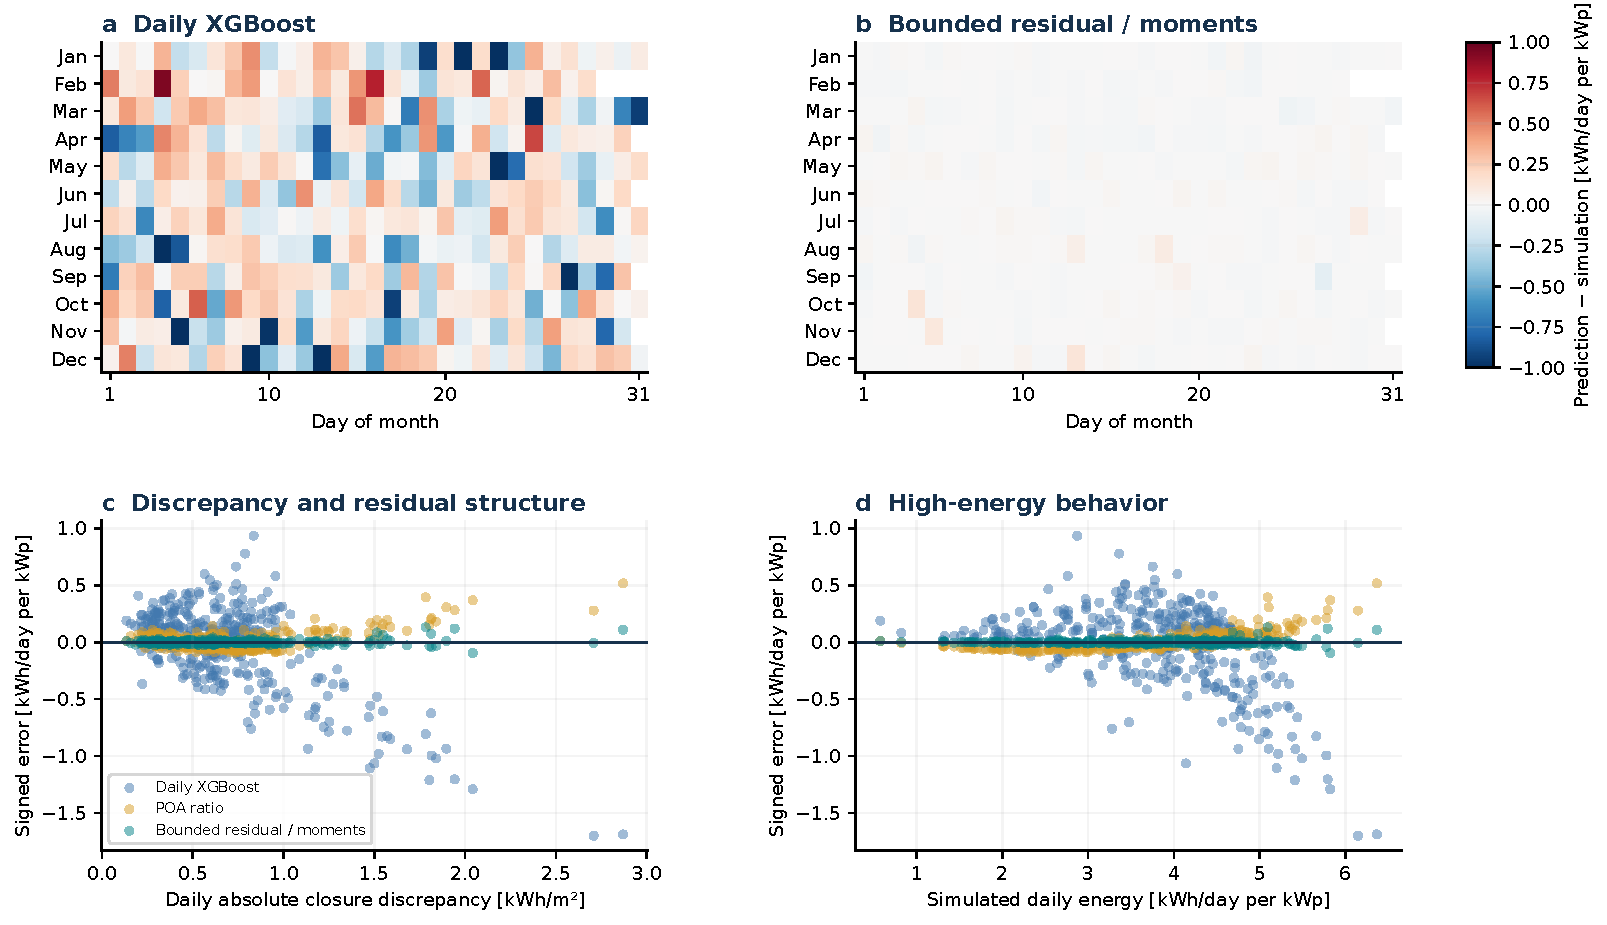
\includegraphics[width=\linewidth]{error-atlas.pdf}
\caption{2025 error atlas. Top: calendar maps of signed error using the same color limits; values outside those limits saturate. Bottom: signed errors against absolute closure discrepancy and simulated daily energy. Blank calendar cells are nonexistent dates. Each point represents one day, and both axes use the computed simulation or its input diagnostics.}\label{fig:atlas}\end{figure}

Figure~\ref{fig:ablation} separates representation from residual parameterization. Supplying POA information to a residual learner lowers MAE from 0.26115 for daily-weather XGBoost to 0.01613. Adding the irradiance-intensity, temperature and wind moments lowers it further to 0.01049, a 35.0\% reduction relative to the residual/POA variant. The moments are introduced together, so the experiment does not identify the individual contribution of each moment.

Adding both closure statistics to the moment-based residual model gives MAE 0.01090. It is slightly worse than the simpler moment model in both validation RMSE and 2025 MAE. Closure remains useful as an audit statistic but is not supported as a necessary predictor here. The closure-augmented direct model has MAE 0.01869, compared with 0.01961 without closure. Thus the feature's apparent value depends on the response parameterization, and its inclusion cannot be justified solely by the daily-weather model's residual pattern.
\begin{figure}[htbp]\centering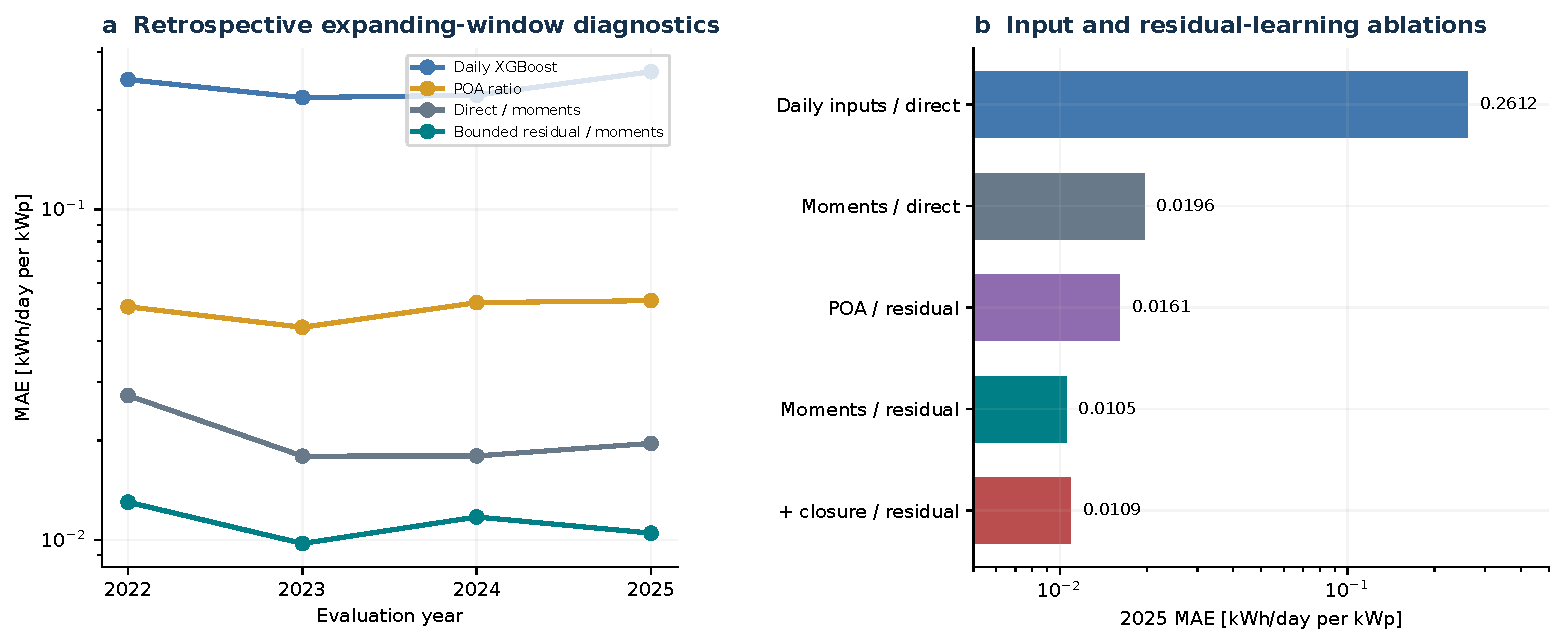
\includegraphics[width=\linewidth]{ablation.pdf}
\caption{Representation and fitting diagnostics. (a) Expanding-window MAE with settings selected on 2024; earlier windows are retrospective. (b) 2025 input and residual-learning ablations. Logarithmic axes retain visibility of differences at the smaller error scales.}\label{fig:ablation}\end{figure}

\subsection{Regime performance and historical stability}
Table~\ref{tab:regimes} and Figure~\ref{fig:sensitivity}(b) report the predefined regime results. Daily-weather XGBoost has MAE approximately 0.160 in the low-closure group and 0.381 in the high-closure group. The proposed model retains substantially lower error in all three groups, as well as on rainy and hot days. These comparisons support the usefulness of the expanded representation under varied inputs, without showing that closure discrepancy causes the error or that the groups are interchangeable across sites.
\begin{table}[htbp]\centering\small
\caption{Regime MAE in 2025 (\unit{}). Thresholds are computed from 2021--2024. Rain and temperature groups overlap the closure groups.}\label{tab:regimes}
\begin{tabular}{@{}lrrrr@{}}\toprule
Regime & Days & Daily XGBoost & POA ratio & Proposed\\\midrule
Low closure discrepancy & 93 & 0.15997 & 0.03443 & 0.00834 \\
Middle closure discrepancy & 124 & 0.19455 & 0.03842 & 0.00884 \\
High closure discrepancy & 148 & 0.38054 & 0.07689 & 0.01323 \\
Precipitation $\geq10$ mm & 92 & 0.23157 & 0.04417 & 0.00979 \\
Temperature $>$ training 90th percentile & 40 & 0.29400 & 0.07352 & 0.01219 \\
\bottomrule\end{tabular}\end{table}

The proposed model's historical-window MAE ranges from 0.00976 to 0.01302. The POA ratio and daily-weather XGBoost remain less accurate in these windows. Because the 2024 selection period informed the settings used in earlier windows, this result is evidence of retrospective consistency, not a substitute for nested external validation.

\subsection{Irradiance intervention}
The intervention in Eq.~\eqref{eq:intervention} changes the simulated 2025 annual energy from 1,369.08 to 1,405.97 kWh/kWp, an increase of 2.69\%. Table~\ref{tab:intervention} and Figure~\ref{fig:sensitivity}(a) show the corresponding approximation errors. Daily-weather XGBoost becomes much more accurate when trained and evaluated against the modified reference. That result shows that reference construction changes the difficulty of the learning problem; it does not establish that the modified reference is closer to actual production.
\begin{table}[htbp]\centering\small
\caption{Effect of the DNI intervention. Both the simulated target and its predictors are recomputed, and each model is refitted using its previously selected settings. MAE is in \unit{}.}\label{tab:intervention}
\begin{tabular}{@{}lrrr@{}}\toprule
Reference construction & Daily XGBoost & POA ratio & Proposed\\\midrule
Downloaded components & 0.26115 & 0.05300 & 0.01049 \\
Algebraic DNI intervention & 0.03312 & 0.03733 & 0.00805 \\
\bottomrule\end{tabular}\end{table}
\begin{figure}[htbp]\centering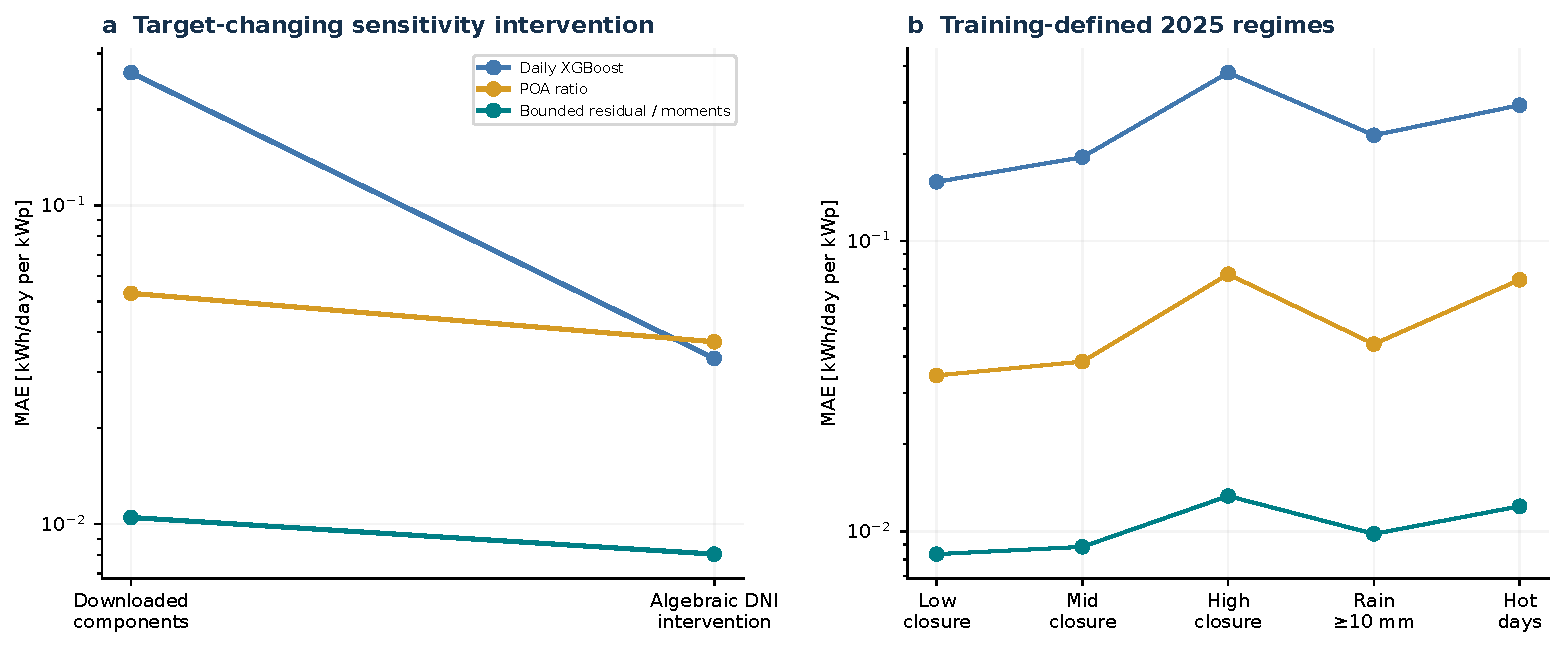
\includegraphics[width=\linewidth]{sensitivity.pdf}
\caption{Input diagnostics and sensitivity. (a) Error against each of two different reference constructions; the connected values are not errors against a common ground truth. (b) MAE within training-defined closure, precipitation and temperature regimes in 2025.}\label{fig:sensitivity}\end{figure}

\section{Discussion}
\subsection{What the experiment establishes}
The principal finding is an input-information effect followed by a smaller, measurable residual-learning effect. Daily-weather models compress 24 hourly records into a handful of means and totals. A deterministic converter does not generally commute with that aggregation: irradiance transposition, thermal response, optical losses and inverter conversion operate before daily summation. The proposed moments retain selected interactions that otherwise disappear. Their usefulness is supported by the reduced residual/POA ablation, while the matched-input direct model isolates the additional benefit of learning around a calibrated anchor.

The exceptionally high $R^2$ of the proposed model must be interpreted in that setting. Its inputs include POA information from the same optical calculation that supports the reference. This is an intentional emulation design, not evidence that the method predicts field production with comparable accuracy. The target and predictors share a deterministic physical construction. Such agreement can help test representation choices and build simulator surrogates, but it supplies no independent evidence about roof geometry, weather representativeness or installed-system behavior.

The moment and closure ablations also constrain the methodological claim. The data do not support adding every available physical diagnostic. The simpler moment representation has the better validation score, and the closure-augmented residual variant does not improve evaluation MAE. Nor is a new optimization algorithm introduced: the learner is standard regularized boosting. The contribution lies in the physical representation, the anchored bounded formulation and the controlled experiment that separates their effects.

\subsection{Computational interpretation}
The approach reuses solar-position and POA calculations and replaces the subsequent conversion mapping with a fitted daily correction. Optical preprocessing therefore remains necessary. The supplied physical simulator already evaluates this small fixed system quickly, and the present extension does not provide a hardware-controlled runtime benchmark. There is no demonstrated end-to-end speed advantage. Training, candidate evaluation and preprocessing would need to be included before any computational benefit could be claimed. Where the original simulator is sufficiently inexpensive, direct simulation remains the appropriate default.

\subsection{Limits and next validation step}
The reference represents a single generic system, one location and five years of gridded weather. No measured photovoltaic output or local radiometer record is available. The analysis therefore cannot establish operational accuracy, forecast skill, regional transferability or the correctness of the DNI intervention. Results may change with array orientation, inverter sizing, thermal assumptions, cloud regimes or source-product versions. Historical windows reuse settings informed by 2024, and bootstrap intervals are conditional on a single evaluation year and fitted model. Architecture development also followed inspection of the earlier benchmark, which limits confirmatory inference.

A meaningful next experiment would freeze the representation and selection rules, then evaluate them on independent sites or a later data period. Measured AC energy, array specifications and local irradiance would permit comparison of the physical simulator, the anchor and residual correction against the same field reference. Future forecasting would additionally require weather forecasts available at issue time; realized same-day weather cannot be substituted for those forecasts. These extensions should precede claims about deployment or superiority to operational forecasting systems.

\section{Conclusion}
A daily photovoltaic emulator can be limited more by the irradiance information retained in its predictors than by the choice between standard learning algorithms. On the supplied Cagayan de Oro archive, a POA anchor with irradiance-intensity, temperature and wind moments reduces 2025 simulation MAE to 0.01049~\unit{}. Direct boosting with the same inputs gives 0.01961, and the POA ratio alone gives 0.05300. The matched-input comparison supports residual learning for this particular emulation problem, while the moment ablation supports preserving selected subdaily interactions.

Closure discrepancies remain diagnostic quantities; adding them does not improve the selected moment-based residual model. Recomputing DNI changes both reference yield and learning difficulty and cannot establish improved physical accuracy. The resulting method and reproducibility package support further simulator and field-validation experiments, with no claim of measured-production accuracy or demonstrated computational savings.

\FloatBarrier
\section*{Declarations}
\paragraph{Funding.} \FundingStatement
\paragraph{Competing interests.} \ConflictStatement
\paragraph{Author contributions.} \ContributionStatement
\paragraph{Ethics and consent.} This study uses public gridded environmental data and simulated photovoltaic outputs. It contains no human-participant or animal experiments and no personal records.
\paragraph{Data availability.} The source weather data are publicly accessible from NASA POWER at \url{https://power.larc.nasa.gov/}. The exact hourly archive, original monthly responses, derived features, daily simulated references, evaluation predictions and result tables accompany this manuscript in the reproducibility package. No measured photovoltaic-production data were used.
\paragraph{Code availability.} The reproducibility package contains the physical reference implementation, training and evaluation code, figure-generation code, software versions, random seeds and execution instructions.\ifdefempty{\RepositoryURL}{}{ The versioned repository is available at \url{\RepositoryURL}.}
\paragraph{Acknowledgment.} The study uses data distributed by the NASA POWER project and the open-source pvlib and XGBoost software packages.

\setlength{\bibsep}{3pt}
\bibliographystyle{abbrvnat}
\begingroup\small
\bibliography{references}
\endgroup
\end{document}
